\chapter{Modularny system symboliczny jako model działania mózgu}
\label{ch:modularity}

Uczenie maszynowe jest pojęciem algorytmicznym, jednak jego rzeczywista implementacja opiera się wyłącznie na najwydajniejszych obliczeniowo dostępnych systemach symbolicznych -- komputerach.
Mózg z kolei jest najbardziej złożonym i potężnym systemem ``silnej inteligencji'' poznanym przez człowieka.
Dlatego jeśli chcemy zestawić jego działanie z uczeniem maszynowym musimy posiadać jakiekolwiek podstawy architektoniczne.
Dopiero podobieństwa systemowe będą punktem wyjścia do podobieństw funkcjonalnych.

Jak się jednak okazuje, nie jest to jednak dużym wyzwaniem.
Istnieje wiele dobrze podpartych powodów by uważać, że model działania mózgu -- podobnie jak komputera -- jest modularnym systemem symbolicznym.

\section{Kognitywistyczne podstawy i rozwój modelu systemu symbolicznego}
\label{cognitive-basics}

Zanim można będzie analizować modularność oraz jej istotne cechy powiązane z topologią modelu systemu symbolicznego przypisanego funkcjonowaniu mózgu, należy wyjaśnić, dlaczego taka właśnie topologia jest z nim wiązana.
W tym celu warto prześledzić drogę ewolucji idei oraz teorii odnoszących się właśnie do tej tematyki.

\subsection{Koneksjonizm}

Jedną z pierwszych teorii wiązanych z mózgiem jako systemem symbolicznym był koneksjonizm.
Wyjaśnia on poznanie jako proces wynurzający się ze wzajemnego działania i współpracy pomiędzy podstawowymi elementami przetwarzającymi \cite{bechtel1993case}.

Jest on istotny w ramach omawianego aspektu, gdyż był podstawą teoretyczną abstrakcji działania mózgowych połączeń neuronalnych, która finalnie doprowadziła do pierwszych modeli sztucznych sieci neuronowych.
Jeszcze sam Alan Turing, ojciec informatyki i sztucznej inteligencji, proponował utworzenie architektury komputerowej opartej na jednostki podobne neuronom \cite{copeland1996alan}.

Koneksjonistyczna idea działania poznania sugeruje, że taka abstrakcja -- mimo, że nie oddaje szczegółów działania biologicznego mózgu -- utrzymuje naturę działania mózgu, funkcje poznawcze.
Jak jednak zostało już opisane i zaznaczone w rozdziale \hyperref[chapter1]{rozdziale \ref*{chapter1}}, szybko okazało się, że takie powiązanie okazuje się być znacznie bardziej skomplikowane i złożone.

\subsection{Kognitywizm}

Na koneksjonistyczne problemy modelowania działania mózgu odpowiada kognitywizm.
W tym podejściu poznanie definiuje się jako manipulację symbolami formalnymi, gdzie wnioskowanie opiera się na manipulacji reprezentacjami symbolicznymi odpowiadającymi informacji o środowisku otrzymanej przez percepcję.
Formalizacją takiego ujęcia była hipoteza systemu symboli fizycznych \cite{newell1981computer}, w której to taki system symboli fizycznych jest jednocześnie niezbędny oraz wystarczający dla inteligentnego zachowania.

Takie podejście okazało się być bardziej zbliżone działaniu mózgu, pomogło w pierwszej fazie uformować się kognitywistyce oraz dało początek niektórym sztucznym architekturom kognitywnym opartym na regułach, takie jak SOAR \cite{laird2019soar}\footnotemark.
\footnotetext{
	Projekt SOAR jest do teraz aktywnie rozwijany.
	Szczegółowe informacje na jego temat znajdują się na oficjalnej stronie: \url{https://soar.eecs.umich.edu}.
	Repozytoria związane z projektem są otwartoźródłowe i znajdują się w serwisie GitHub: \url{https://github.com/SoarGroup}.
}
Ponownie jednak taka architektura okazała się nie oddawać w pełni złożoności działania poznania u człowieka.

\subsection{Modelowanie probabilistyczne}

W ludzkim poznaniu, a co za tym idzie w modelu działania mózgu, informacje czy samo wnioskowanie nie opiera się wyłącznie na Boole'owskiej prawdzie i fałszu, tak, jak ma to miejsce w logice pierwszego stopnia, na której oparte były poprzednie architektury.
Zazwyczaj człowiek nie jest ``pewny'', ale ``przekonany''.
Umysł operuje na zdarzeniach natury indukcyjnej i pewność nigdy nie jest rzeczywiście niepodważalna.
Nie brnąc dalej w filozoficzną tematykę czym jest prawda i fałsz, wydaje się być oczywistym, że człowiek działa raczej na zasadzie prawdopodobieństw i nieokreśloności.

Matematyka jednak również była tutaj w stanie pomóc, jako, że logika probabilistyczna była już dostępna i dobrze rozwinięta.
Architektury modelujące oparte na kwantyfikacji stanu świata w terminach stopnia prawdziwości nazywanej teorią probabilistyczną \cite{jaynes1988does}, zbliżyły się jeszcze bardziej do poznania człowieka i modelowania działania ludzkiego mózgu.
Takie podejście jest podstawą wyjaśniania podejmowania optymalnych decyzji wykonywanych w warunkach niepewności.
Są postulaty wskazujące na to, że na poziomie algorytmicznym mózgi wykorzystują algorytmy wnioskowania przybliżonego (\emph{approximate inference}) \cite{andrieu2003introduction} tak, aby wytwarzać wystarczająco dobre rozwiązania dla szybkiego i oszczędnego podejmowania decyzji.

\subsection{Oddolna emergencja a odgórna abstrakcja}

Jeśli zaczniemy rozważania od odwrotnej strony przy pomocy pytania: ``jaki system sztucznie inteligenty byłby najbliższy działania rzeczywistego, biologicznego mózgu'' szybko dotrzemy do wniosku, że byłaby to jego symulacja.
Taki system oparty by był na \emph{oddolnej emergencji} (\emph{bottom-up emergence}), gdzie zachowania i poznanie symulowanego mózgu wyłoniłoby się z symulacji najprostszych jednostek, neuronów oraz ich środowiska.
Jednak jak twierdzi badacz, który zajmował się symulacją systemów wzgórzowo-korowych u ssaków \cite{izhikevich2008large} Eugene Izhikevich, nawet symulacja sekundy działania całego ludzkiego mózgu nie przyczyniłaby się znacząco do neuronauki \cite{Izhikevich2006why}.
Dodając do tego ogrom skali zadania, jakim jest symulacja ludzkiego mózgu można zrozumieć, dlaczego zwrócono się w stronę alternatywnego podejścia.

Rozwój podejść z kategorii \emph{odgórnej abstrakcji} (\emph{top-down abstraction}) jest obrazowany przez poprzednie tematy z \hyperref[cognitive-basics]{tej sekcji}.
Te algorytmy są obliczeniowo wykonywalne i dzięki temu mają potencjał użytkowy do analiz teoretycznych.
Obiecującym punktem powstałym na wyjściu implementacji założeń teoretycznych w praktyce są sztuczne sieci neuronowe, podstawa nowoczesnego głębokiego uczenia i dużej porcji całego uczenia maszynowego.
Można je wiązać z poziomem biofizycznym -- głównym źródłem porównań przy oddolnej emergencji -- jako abstrakcje biologicznych sieci neuronów opartych na częstotliwości (\emph{rate-based}) \cite{dayan2001theoretical}.
Architektury sieci mogą być wytwarzane w procesie ewolucyjnym, czy algorytmów bazowanych na strategiach ewolucyjnych \cite{real2017large}.
Są zgodne również z modelowaniem probabilistycznym, jak zauważono, algorytmy obliczeniowe powstałe w wyniku uczenia są zbliżone efektywnie do wnioskowania bayesowskiego \cite{gal2016dropout, mandt2017stochastic}.
Są związane nawet z bazą komputacjonistycznego podejścia poprzez ugruntowanie reprezentacji symbolicznych w stanach sensorycznych świata rzeczywistego \cite{harnad1990symbol}.

Użycie koneksjonistycznych sztucznych sieci neuronowych wzbogaconych o architektury i struktury innych modelów systemów przetwarzania symbolicznego wydaje się być najbliżej potencjalnej inteligencji sztucznej.
Nie jest to jednak jednoznaczne z tym, że są także najbliżej odwzorowywania działania mózgu.
Aby móc wyciągać takie wnioski należy wykazać także, że mózg również można zaliczyć do kategorii systemów symbolicznych o topologii choćby zbliżonej do wymienionych.
W tym warto wspomnieć i bardzo istotnej cesze sztucznych systemów symbolicznych zgodnej z ideą budowania takowych od podstaw \cite{bechtel1993case} : \emph{modularność}.

\section{Zestawienie modularności mózgu z modularnością sztucznych systemów symbolicznych}

Intuicyjne czujemy, że sztuczne systemy symboliczne -- czyli w rzeczywistych implementacjach po prostu komputery -- są modularne.
Dodatkowo dla osób związanych bliżej z architekturą komputerową, w tym w szczególności architekturą oprogramowania, oczywista jest prawdziwość takiego sformułowania również w kontekście programów, czyli funkcjonalnością systemową.
Z kolei jedną z pierwszych rzeczy przyswajanych przy uczeniu się neurobiologii jest podział mózgu na pola Brodmanna, które również można interpretować jako swoistą modularność.
Mimo wszystko te tezy warto przeanalizować dokładniej, gdyż pojawia się tu więcej istotnych cech wspólnych niż może się to wydawać.

\subsection{Modularność uczenia maszynowego i systemów symbolicznych}

Nowoczesne architektury rozwiązań pojawiających się w dziedzinie uczenia maszynowego mają dodatkowo cechę wyłaniającą się wraz ze wzrostem złożoności systemów -- modularność.

Jej wartość w uczeniu głębokim oraz szerzej pojętych sieciach neuronowych zauważana była już od dłuższego czasu \cite{schmidt1998modularity}.
Co więcej, istnieją powody by wierzyć, że taka struktura jest w pewnym sensie optymalna.
Gdy klasyfikator nieliniowy o budowie modularnej jest poddawany ``procesowi ewolucji'' poprzez aplikowanie szumu do jego wag wewnętrznych, topologia modularna sieci ewoluuje bez wsparcia reprezentacjonalnego \cite{hoverstad2011noise}.

Analizując jako przykład biliniowe konwolucyjne sieci neuronowe (B-CNN) \cite{lin2015bilinear} taką modularność można wyraźnie dostrzec nawet w jednej jednostce sieciowej.
Składa się ona bowiem z czterech kluczowych komponentów:
\begin{itemize}
	\item Dwóch niezależnych strumieni konwolucyjnych służących jako \emph{ekstraktory cech};
	\item Operatora nakładania biliniowego (bilinear pooling) agregującego wyniki strumieni konwolucyjnych do wektora biliniowego;
	\item Głębokiej sieci neuronowej z gęsto łączonymi warstwami służącej za \emph{klasyfikator}.
\end{itemize}
Można więc stwierdzić, że taka sieć neuronowa jest \emph{modularna}. Składa się z połączonych komponentów (modułów), z których każdy jest wyspecjalizowany do konkretnego zadania.
Dodatkowo można zauważyć naturę tej modularności -- jest ona \emph{hierarchiczna}.
Część sieci odpowiedzialna za ekstrakcję cech obrazu składa się z trzech modułów: dwie sieci konwolucyjne działające niezależnie oraz operator agregujący ich wyniki.

Dodatkowo w wykorzystaniu praktycznym takich czy innych sieci czy rozwiązać uczenia maszynowego pojedynczy system traktuje się właśnie jako moduł, którego zadaniem jest wykonanie wymaganej czynności.
Jest to moduł wyspecjalizowany w tym co robi.
Tak tutaj, w przypadku B-CNN jej zadaniem jest klasyfikacja obrazu.
System, który ją wykorzystuje również może być -- a nawet zazwyczaj jest -- modułem.
Przykładowo możemy wyobrazić sobie funkcję wyszukiwarki za pomocą obrazu, która wykorzystuje moduł B-CNN aby skategoryzować obraz, a następnie inne moduły aby wyszukać obrazy z odpowiedniej kategorii.

Taki sposób działania sztucznych systemów symbolicznych jest dość uniwersalny i nazywa się \emph{hierarchiczną modularnością}.
Jest on nieodłącznym elementem informatyki, pozwala na budowanie bardzo złożonych systemów poprzez enkapsulację funkcjonalności.
Co więcej, już prawie 60 lat temu argumentowano, że każdy złożony system jest zorganizowany w sposób hierarchiczny, niezależnie, czy jest on społeczny (np. system transportowy), czy jest fizycznym systemem symbolicznym czy nawet biologicznym \cite{simon1962architecture}.

\subsection{Modularność mózgu}

Istnieją prace analizujące modularność mózgu.
Jak się okazuje, modularność ta nie jawi się wyłącznie w różnicach cytoarchitektonicznych, które pozwoliły wyodrębnić obszary nazywane polami Brodmanna.
Jawi się ona także na ``wyższym poziomie'' abstrakcji, w sieciach funkcjonalnych.
Przeprowadzone analizy wykazały, że w wyniku podziału modularnego powstają spójne sieci topologiczne \cite{bullmore2009complex}.
Niedawno rozpoczęto także badania nad charakterem tej modularności.
Co istotne w tej tematyce, zaczęto badać czy jest ona hierarchiczna, tak, jak przewidywał to Simon względem każdego systemu złożonego \cite{simon1962architecture}.
Jak się okazuje, pierwsze próby wyodrębnienia takiej hierarchii modularnej sieci funkcjonalnych mózgu zakończyły się pozytywnymi wynikami \cite{meunier2009hierarchical}.

Dane z przeprowadzonego badania fMRI przetworzono metodą Louvain do detekcji wspólnot.
Wynikiem takiego przetworzenia był wielowarstwowy graf modułów funkcjonalnych, w którym warstwy odpowiadają hierarchii przynależnościowej pod-modułów do modułów wyższego rzędu.
Analiza wyodrębniła pięć największych obszarów (modułów) najwyższego poziomu, do których dodatkowo można przyporządkować funkcje bazując na znajomości funkcji obszarów mózgowych znajdujących się w obrębie danego modułu.
Podział ten przedstawia \hyperref[fig:brain-functional-modules]{rysunek \ref*{fig:brain-functional-modules}}.

\begin{figure}[t]
	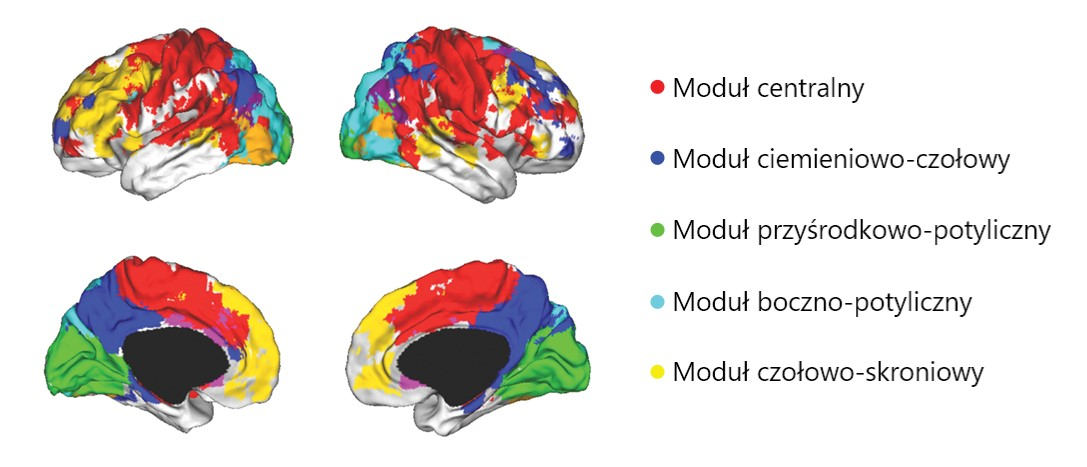
\includegraphics[width=\textwidth]{Images/BrainFunctionalModules}
	\caption{Moduły najwyższego poziomu hierarchii modularnej sieci funkcjonalnych mózgu}
	Rysunek zaadoptowany z pracy autorów \cite{meunier2009hierarchical}.
	Pokazuje obszary pięciu największych modułów trzeciej (najwyższej) hierarchii.
	\label{fig:brain-functional-modules}
\end{figure}

Mimo niewielkiej ilości tych modułów najwyższego rzędu można dostrzeć pewne prawidłowości.
Jak widać na szczegółowych danych w \hyperref[tab:modular]{tabeli \ref*{tab:modular}}, przynależność do stopnia hierarchii nie jest równoznaczna z wielkością modułu.
Na najwyższym poziomie wyodrębniono osiem obszarów, z czego tylko pięć wspomnianych było wystarczająco złożonych by móc podlegać dalszej analizie.

\begin{table}[ht]
	\begin{center}
		\begin{tabular}{  c | c | c   }
			\hline
			Moduł & Liczba węzłów & Liczba pod-modułów \\
			\hline
			\hline
			\begin{tabular}{@{}c@{}} Centralny \\ (sensomotoryczny) \end{tabular} & 239 & 11  \\[1em]
			\begin{tabular}{ @{}c@{}} Ciemieniowo-czołowy \\  (główny/uwagowy) \end{tabular} & 138 & 10  \\[1em]
			\begin{tabular}{@{}c@{}} Przyśrodkowo-potyliczny \\ (pierwszorzędowy wizualny) \end{tabular} & 132 & 1 \\[1em]
			\begin{tabular}{@{}c@{}} Boczno-potyliczny \\ (drugorzędowy wizualny) \end{tabular} & 101 & 1 \\[1em]
			\begin{tabular}{@{}c@{}} Czołowo-skroniowy \\ (symboliczny) \end{tabular} & 89 & 24 \\
			\hline
		\end{tabular}
	\end{center}
	\caption{Moduły najwyższego poziomu hierarchii sieci funkcjonalnych mózgu}
	Tabela zaadoptowana z pracy autorów \cite{meunier2009hierarchical}.
	Przedstawia ilość węzłów znajdujących się wewnątrz każdego z największych modułów najwyższego poziomu hierarchii oraz ilość znajdujących się w nich pod-modułów.
	\label{tab:modular}
\end{table}

Największy z nich to moduł centralny, \emph{somatosensomotoryczny}.
Jest on jednocześnie dobrym przykładem, że podział modularny zachowywał właściwości podziału funkcjonalnego także na niższych warstwach hierarchii.
Zawarte w module centralnym kora przyśrodkowa oraz kora boczna znalazły się bowiem w osobnych pod-modułach.
Co więcej -- idąc głębiej, w module drugiego poziomu zawierającego korę boczną obszary przedśrodkowe oraz zaśrodkowe były odseparowane od górnej kory skroniowej.

Moduł ciemieniowo-czołowy, drugi pod względem ilości zawartych w sobie węzłów, obejmował obszary funkcjonalnie odpowiadające części mózgowych \emph{głównej} oraz \emph{uwagowej}.
On wraz z poprzednio wymienionym modułem są stosunkowo zrównoważone.
Posiadają one liczbę pod-modułów, która nie odbiega od normy.
Wśród nich jest niewielka ilość dużych pod-modułów i wiele małych.

Następny co do wielkości moduł przyśrodkowo-potyliczny zawiera w sobie pierwszorzędową korę wzrokową, stąd funkcjonalnie przyporządkowany jest jako moduł \emph{pierwszorzędowy wizualny}.
Jeszcze następny -- obszar boczno-potyliczny -- nazwany został modułem \emph{drugorzędowym wizualnym} z powodów analogicznych do wcześniejszego.
Wymienione zostały przeze mnie razem, gdyż dzielą poza faktem, że funkcjonalnie odnoszą się do obszarów wizualnych, dzielą ze sobą jeszcze jedną istotną cechę -- oba posiadają wyłącznie jeden pod-moduł.

Ostatni moduł najwyższego poziomu z tych wartych analizy, czołowo-skroniowy, został nazwany \emph{symbolicznym}.
Podobnie jak inne, nazwa ta została wyciągnięta z określenia, jakim można by było skategoryzować funkcjonalnie obszary w nim zawarte.
On również wyróżnia się spośród pozostałych, ale w kierunku przeciwnym do modułów wizualnych.
Posiada bardzo dużą liczbę pod-modułów o stosunkowo równej wielkości.

Wspomniane prawidłowości oraz różnice między-modularne tworzą dość spójny obraz modularności hierarchicznej w funkcjonalnych sieciach mózgowych.
Modularność jest wyraźna nawet bazując na samej analizie funkcjonalnej oraz spójności powstałych obszarów, dodatkowo potwierdzone przeprowadzonym przez autorów porównaniem, w którym powstała modularność była wyższa niż dla sieci generowanych losowo.
Hierarchiczność również jest zauważalna i dodatkowo mówi nam dużo o naturze tych wyodrębnionych obszarów funkcjonalnych.
Warte spostrzeżenia jest, że te wnioski są zbieżne z analogicznymi sztucznymi systemami symbolicznymi oraz ich topologią.
Obszary wizualne, podobnie jak wykorzystywane w rozwiązania w systemach widzenia maszynowego opierają się na jednej, wysoce złożonej i ``uniwersalnej'' sieci odpowiedzialnej za wyodrębnienie istotnych informacji z otoczenia.
Obszary symboliczne natomiast składają się z wielu małych, ale wysoce wyspecjalizowanych modułów współpracujących w przetwarzaniu informacji.
